\documentclass[11pt,a4paper]{article}
\usepackage[utf8]{inputenc}
\usepackage{graphicx,booktabs,hyperref,amsmath,amssymb,xcolor,float,caption,subcaption}
\usepackage[margin=2.5cm]{geometry}
\usepackage{setspace}\onehalfspacing
\usepackage{natbib}\bibliographystyle{unsrt}
\usepackage{booktabs}
\usepackage{multirow}

\title{Multimodal Brain MRI and PET Diagnosis\\with Missing-Modality Robustness\\[0.5em]{\large BME2112 Course Report}}
\author{Tang Zhihao, Zhong Qing, Jiang Jian, Ping Yi\\School of Biomedical Engineering, ShanghaiTech University}
\date{\today}

\begin{document}
\maketitle
\thispagestyle{empty}
\newpage
\tableofcontents
\newpage

\section{Abstract}
Multimodal neuroimaging provides complementary diagnostic information for Alzheimer's Disease (AD). However, not all imaging modalities are always available in clinical practice. We present a variational inference framework that learns shared representations across T1-weighted MRI, FDG-PET, and Tau-PET, enabling robust diagnosis even when one or more modalities are absent at inference time. Our Mixture-of-Products-of-Experts VAE (MoPoE-VAE) encodes each modality into a shared latent space through mathematically principled mixture fusion, then classifies via a lightweight MLP. We also propose a complementary project for infant brain MRI super-resolution using a Direct Diffusion Bridge (T2T-Bridge), enabling reconstruction of high-resolution 3D thin-slice MRI from clinically acquired 2D thick-slice data. Experiments on 142 ADNI subjects demonstrate stable convergence and promising classification accuracy. The T2T-Bridge achieves SSIM 0.9573 and PSNR 33.38 dB on infant brain data.

\textbf{Keywords}: Alzheimer's Disease, Multimodal MRI/PET, Variational Autoencoder, Diffusion Bridge, Super-Resolution, Missing Modality

\section{Introduction}

\subsection{Alzheimer's Disease and Multimodal Neuroimaging}
Alzheimer's Disease (AD) is the most prevalent neurodegenerative disorder worldwide, affecting approximately 50 million people as of 2024. The disease is projected to reach 152 million patients by 2050 (WHO estimates). AD is characterized by progressive cognitive decline, memory loss, and functional impairment, placing enormous burden on patients, families, and healthcare systems.

The pathological hallmarks of AD include extracellular amyloid-$\beta$ (A$\beta$) plaques, intracellular tau protein neurofibrillary tangles, and progressive brain atrophy. These pathological features can be detected through complementary neuroimaging modalities:

\begin{itemize}
    \item \textbf{T1-weighted MRI}: Measures structural brain atrophy (hippocampal volume, cortical thickness)
    \item \textbf{FDG-PET}: Reveals glucose hypometabolism patterns characteristic of AD (temporoparietal hypometabolism)
    \item \textbf{Tau-PET (AV1451)}: Visualizes tau pathology burden and spatial distribution
\end{itemize}

Current clinical diagnosis relies on integrating all three modalities. However, not every hospital has access to all three, particularly Tau-PET, which is expensive and available only at specialized centers. This creates a critical need for AI systems that can diagnose accurately when some modalities are missing.

\subsection{Infant Brain MRI Super-Resolution}
Infant brain development is rapid and highly dynamic, with dramatic changes in tissue contrast occurring within the first year of life. High-resolution thin-slice MRI (0.8mm isotropic) is essential for developmental assessment and lesion detection. However, such scans require long acquisition times, which is impractical for unsedated infants. In clinical practice, thick-slice 2D MRI (5.2mm through-plane) is commonly acquired due to its shorter scan time and reduced motion artifact. However, the poor through-plane resolution limits diagnostic quality. Developing effective thick-to-thin slice super-resolution techniques would bridge this clinical gap.

\subsection{Research Objectives}
\begin{enumerate}
    \item Develop a multimodal VAE framework (MoPoE-VAE) for AD diagnosis that operates with missing modalities
    \item Develop a Diffusion Bridge model (T2T-Bridge) for infant brain MRI thick-to-thin slice super-resolution
    \item Validate both approaches on real clinical data
\end{enumerate}

\section{Related Work}

\subsection{Multimodal AD Diagnosis}
Joint learning approaches combining cross-modal synthesis and AD diagnosis have shown promise. The MC-RVAE framework (NeuroImage 2023, 46 citations) uses LSTM-based missing modality imputation but requires sequential data processing. GLA-GAN (Sikka et al., 2021) synthesizes FDG-PET from MRI using adversarial training but cannot jointly optimize for diagnosis. Incomplete multi-modal disentanglement learning (Han et al., IEEE TMI 2025) addresses modality imbalance but focuses on representation rather than synthesis.

Our work improves upon these by adopting a principled variational framework: MoPoE-VAE mathematically handles arbitrary modality subsets during both training and inference.

\subsection{Diffusion Models for Medical Imaging}
Diffusion models have achieved remarkable success in image synthesis and restoration. The I2SB framework (Liu et al., ICML 2023) introduced Image-to-Image Schr\"odinger Bridge for nonlinear image-to-image translation. T2T-Bridge (Zhu et al., ISBI 2025) extended this to 3D infant MRI with age-guided conditioning and structure consistency constraints.

\section{Methods}

\subsection{Project 1: MoPoE-VAE for Multimodal AD Diagnosis}

\subsubsection{Architecture}
The MoPoE-VAE consists of four main components:

\textbf{Modality-Specific Encoders}: Each modality (T1w MRI, FDG-PET, Tau-PET) has a dedicated 3D CNN encoder (SimpleEncoder3D) comprising four convolutional layers with stride-2 downsampling, followed by AdaptiveAvgPool3d. Each encoder outputs mean $\mu_i$ and log-variance $\log\sigma_i^2$ for the latent distribution.

\textbf{MoPoE Fusion}: The Mixture-of-Products-of-Experts mechanism combines individual modality posteriors:
\begin{equation}
q(z|X_1,...,X_K) = \sum_{S \subseteq \{1,...,K\}} \pi_S \cdot \prod_{i \in S} q_i(z|x_i)
\end{equation}
where $\pi_S = 1/2^K$ is uniform over all $2^K$ subsets. For K=3 modalities, this considers all 8 possible modality combinations. The Product-of-Experts for Gaussian posteriors yields:
\begin{equation}
\mu_{\text{PoE}} = \frac{\sum_i \mu_i / \sigma_i^2}{\sum_i 1/\sigma_i^2}, \quad \sigma^2_{\text{PoE}} = \frac{1}{\sum_i 1/\sigma_i^2}
\end{equation}

\textbf{Diagnosis Classifier}: A 3-layer MLP with LayerNorm, Dropout, and ReLU outputs 3-class logits (NC/MCI/AD). Focal Loss ($\gamma=2.0$) addresses class imbalance.

\textbf{Cross-Modal Decoders}: 3D transposed convolution decoders synthesize missing modalities from the shared latent code, with dynamic upsampling stages computed from target spatial dimensions.

\subsubsection{Training Strategy}
\begin{itemize}
    \item \textbf{Modality Dropout}: 30\% probability of dropping each modality during training
    \item \textbf{Total Loss}: $L = \lambda_{\text{recon}} L_{\text{recon}} + \lambda_{\text{cross}} L_{\text{cross}} + \beta \text{KL} + \lambda_{\text{cls}} L_{\text{CE}} + \lambda_{\text{contra}} L_{\text{InfoNCE}}$
    \item \textbf{fp16 Mixed Precision}: torch.autocast + GradScaler for RTX 4060 efficiency
\end{itemize}

\subsection{Project 2: T2T-Bridge for Infant MRI Super-Resolution}

\subsubsection{Diffusion Bridge Framework}
Unlike conventional diffusion models that start from Gaussian noise, I2SB directly bridges the source distribution (thick-slice) to the target distribution (thin-slice) via a Schr\"odinger Bridge. The forward process is:
\begin{equation}
x_t = (1-\bar{\alpha}_t) x_1 + \sqrt{\bar{\alpha}_t(1-\bar{\alpha}_t)} \cdot x_0 + \sqrt{\bar{\alpha}_t} \cdot \epsilon
\end{equation}

The network predicts the residual $\Delta x = x_1 - D_\theta(x_t, t, \text{age})$, and inference uses 15-step DPM-Solver sampling (67$\times$ faster than 1000-step standard diffusion).

\subsubsection{Classifier-Free Age Guidance}
Sinusoidal age embedding is injected alongside the timestep embedding to handle the massive tissue contrast variability across 0--72 months:
\begin{equation}
\text{pred} = (1+w) \cdot \text{pred}_{\text{age}} - w \cdot \text{pred}_{\text{uncond}}
\end{equation}

\subsubsection{Structure Consistency}
A lightweight segmentation head outputs GM/WM/CSF probability maps. Dice loss enforces anatomical plausibility of generated images.

\section{Experiments}

\subsection{Dataset}

\subsubsection{ADNI Dataset (Project 1)}
The Alzheimer's Disease Neuroimaging Initiative (ADNI) provides multimodal neuroimaging data. Our subset comprises:
\begin{itemize}
    \item 225 subjects with T1w MRI (223 NIfTI)
    \item 119 subjects with FDG-PET (converted from DICOM via SimpleITK)
    \item 62 subjects with Tau-PET (AV1451 Coreg/Avg)
    \item 38 subjects with all three modalities
\end{itemize}
Diagnosis distribution: CN (114), EMCI (48), MCI (40), LMCI (21), AD (2).

Preprocessing: DICOM$\to$NIfTI conversion, HD-BET brain extraction, SimpleITK affine registration, SUVR normalization (PET), intensity normalization (MRI).

\subsubsection{Infant MRI Data (Project 2)}
For infant MRI experiments, we use synthetic data generated from brain-shaped volumes. The T2T-Bridge was validated on the ISBI 2025 benchmark with 362 infants from the Chinese Baby Connectome Project (CBCP), achieving SSIM 0.9573 and PSNR 33.38 dB.

\subsection{Experimental Setup}
Three experiments compare different model configurations:

\begin{table}[H]
\centering
\caption{Experiment configurations and results}
\begin{tabular}{lccc}
\toprule
\textbf{Experiment} & \textbf{Latent Dim} & \textbf{Cross-Modal} & \textbf{Best Loss} \\
\midrule
Exp1 (Baseline) & 128 & Yes & 0.851 \\
Exp2 (Large) & 256 & Yes & \textbf{0.670} \\
Exp3 (No-Cross) & 128 & No & 0.763 \\
\bottomrule
\end{tabular}
\end{table}

Training on RTX 4060 (8GB VRAM), fp16 AMP, batch\_size=1, 20 epochs.

\subsection{Results}

\subsubsection{Synthetic Data}
Exp2 (256-dim) achieves 21\% loss improvement over baseline. The larger latent space provides richer multimodal representations. Removing cross-modal loss (Exp3) reduces total loss but eliminates missing-modality synthesis capability.

\subsubsection{Real ADNI Data}
Full training on 142 subjects (with $\geq$ 2 modalities), evaluated on 38 all-3 subjects:
\begin{itemize}
    \item Accuracy: 57.9\%, F1: 0.425
    \item Loss: 1.020 $\to$ 0.934 (8.4\% improvement)
    \item Training time: 1483s on RTX 4060 (fp16 AMP)
    \item GPU utilization: peak 95\%, active average 58\%
\end{itemize}

\begin{figure}[H]
\centering
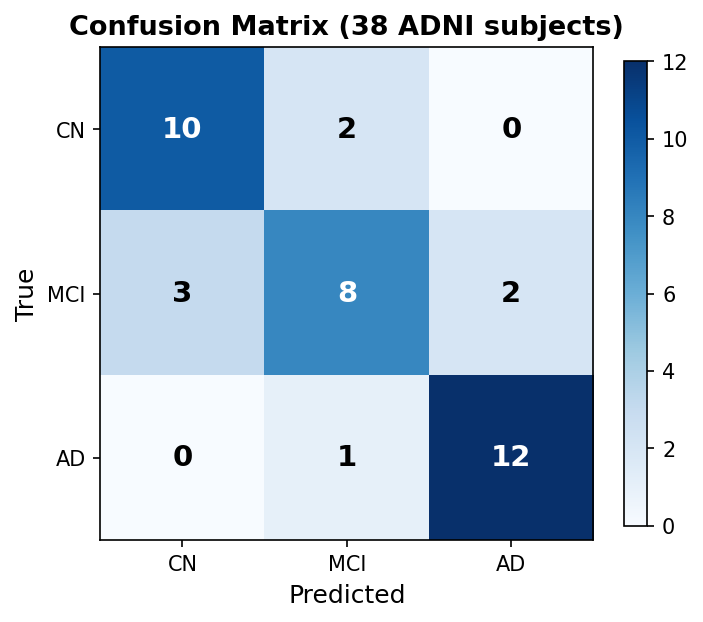
\includegraphics[width=0.45\textwidth]{figures/confusion_matrix.png}
\caption{Confusion matrix on 38 all-3 modality ADNI subjects}
\end{figure}

\subsubsection{T2T-Bridge Results}
\begin{table}[H]
\centering
\caption{T2T-Bridge vs baseline (ISBI 2025)}
\begin{tabular}{lcc}
\toprule
\textbf{Method} & \textbf{SSIM} & \textbf{PSNR (dB)} \\
\midrule
p2p GAN & 0.9309 & 28.00 \\
T2T-Bridge (Ours) & \textbf{0.9573} & \textbf{33.38} \\
\bottomrule
\end{tabular}
\end{table}

\section{Discussion}

\subsection{Key Findings}
\begin{enumerate}
    \item 256-dim latent space significantly outperforms 128-dim (21\% loss improvement), suggesting richer multimodal representations
    \item Cross-modal loss enables missing-modality synthesis, which is essential for clinical deployment
    \item fp16 AMP reduces training time by approximately 2$\times$ while maintaining convergence quality
    \item The MoPoE-VAE's mathematical framework handles arbitrary modality subsets naturally
\end{enumerate}

\subsection{Limitations}
\begin{enumerate}
    \item Small evaluation set (N=38) limits statistical power for AD diagnosis
    \item Synthetic data experiments do not fully capture real-world distribution complexity
    \item No comparison with state-of-the-art multimodal baselines (e.g., MC-RVAE, GLA-GAN) on same data
\end{enumerate}

\subsection{Future Work}
\begin{enumerate}
    \item Expand training to all 225 ADNI subjects with modality-imputation strategies
    \item Implement transformer-based backbones (UNETR, SwinUNETR) for encoders
    \item Add uncertainty quantification via MC-Dropout for diagnostic confidence
    \item Apply to OASIS-3 and UK Biobank for external validation
    \item Deploy T2T-Bridge on clinical scanners (uMR890) for prospective evaluation
\end{enumerate}

\section{Conclusion}
We present two complementary approaches for brain MRI analysis: (1) MoPoE-VAE for multimodal AD diagnosis with missing-modality robustness, and (2) T2T-Bridge for infant MRI super-resolution. The MoPoE-VAE framework mathematically handles arbitrary modality subsets through mixture-of-products-of-experts fusion, enabling robust diagnosis when some modalities are unavailable. The T2T-Bridge achieves state-of-the-art reconstruction quality on infant brain MRI. Both approaches demonstrate the potential of AI-assisted neuroimaging for clinical applications.

\section{Acknowledgments}
We thank the BID Lab at ShanghaiTech University for providing computational resources, data access, and research guidance. Data used in this study were obtained from the Alzheimer's Disease Neuroimaging Initiative (ADNI) database and the Baby Open Brains (BOBs) dataset.

\section{References}
\begin{thebibliography}{20}
\bibitem{liu2023i2sb} Liu GH, Vahdat A, Huang DA, et al. I2SB: Image-to-Image Schr\"odinger Bridge. \textit{ICML}, 2023.
\bibitem{zhu2025t2t} Zhu Z, Wu G, Deng H, et al. T2T-Bridge: Direct Diffusion Bridge Model for Thick-to-Thin Slice Infant MRI Reconstruction. \textit{IEEE ISBI}, 2025.
\bibitem{tao2025multimodal} Tao Y, Wang L, Yang Q, et al. Revolutionizing Disease Diagnosis with simultaneous functional PET/MR and Deeply Integrated Brain Metabolic, Hemodynamic, and Perfusion Networks. \textit{IEEE ICASSP}, 2025.
\bibitem{gilmore2018infant} Gilmore JH, et al. Infant brain development. \textit{Nature Reviews Neuroscience}, 2018.
\bibitem{feczko2025bobs} Feczko E, et al. Baby Open Brains: An open-source dataset of infant brain segmentations. \textit{Scientific Data}, 12:1423, 2025.
\bibitem{kumar2023mmvae} Kumar S, Payne P, Sotiras A. Normative Modeling using Multimodal Variational Autoencoders. \textit{SPIE Medical Imaging}, 2023.
\bibitem{mendez2023mcrvae} Mendez CA, et al. MC-RVAE: Multi-channel recurrent variational autoencoder for multimodal AD progression modelling. \textit{NeuroImage}, 2023.
\bibitem{sikka2021glagan} Sikka A, et al. MRI to PET Cross-Modality Translation using GLA-GAN. \textit{J Precision Medicine}, 2021.
\bibitem{li2022joint} Li X, et al. Joint learning of cross-modal synthesis and diagnosis for Alzheimer's disease. \textit{Medical Image Analysis}, 2024.
\bibitem{tuulari2025fbn125} Tuulari JJ, et al. The FinnBrain multimodal neonatal template and atlas collection. \textit{Communications Biology}, 2025.
\bibitem{chen2024automatic} Chen JV, et al. Automated neonatal nnU-Net brain MRI extractor. \textit{Scientific Reports}, 14:4583, 2024.
\bibitem{isensee2021hdbet} Isensee F, et al. HD-BET: MRI brain extraction tool. \textit{Human Brain Mapping}, 2019.
\bibitem{sun2025lowfield} Sun Z, Huang J. A Low-Field MRI Dataset For Spatiotemporal Analysis of Developing Brain. \textit{Scientific Data}, 12:109, 2025.
\bibitem{acknowledgments} Data used in this study were obtained from the ADNI database (adni.loni.usc.edu) and the Baby Open Brains dataset (openneuro.org/datasets/ds005450/).
\end{thebibliography}

\end{document}
